\paragraph{QuizziPedia::Front-End::Controllers::ResultsController}
\begin{figure} [ht]
	\centering
	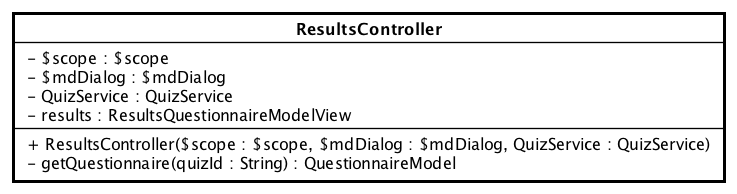
\includegraphics[scale=0.45]{UML/Classi/Front-End/QuizziPedia_Front-end_Controller_ResultsController.png}
	\caption{QuizziPedia::Front-End::Controllers::ResultsController}
\end{figure} \FloatBarrier
\begin{itemize}
	\item \textbf{Descrizione}: questa classe permette di gestire la visualizzazione dei risultati ottenuti dagli utenti che hanno completato il questionario;
	\item \textbf{Utilizzo}: fornisce le funzionalità per recuperare i dati dal back-end e mostrarli all'utente nella view;
	\item \textbf{Relazione con altre classi}:
	\begin{itemize}
		\item \textit{IN} \texttt{ResultsQuestionnaireModelView}: classe di tipo modelview la cui istanziazione è contenuta all'interno della variabile di ambiente \$scope di \textit{Angular.js\ped{G}}. All'interno di essa sono presenti le variabili e i metodi necessari per il \textit{Two-Way Data-Binding\ped{G}} tra la view \texttt{ResultsView} e il controller \texttt{ResultsController}; 
		\item \textit{IN} \texttt{QuizService}: questa classe permette di ottenere i dati di un quiz tramite delle parole chiave inserite dall'utente nella barra di ricerca;
		\item \textit{IN} \texttt{QuestionnaireModel}: rappresenta un questionario. Contiene tutte le informazioni necessarie alla presentazione del contenuto del questionario;
	\end{itemize}
	\item \textbf{Attributi}:
	\begin{itemize}
		\item \texttt{-} \texttt{\$scope: \$scope} \\
		Campo dati contenente un riferimento all’oggetto \$scope creato da \textit{Angular\ped{G}}, viene utilizzato come mezzo di comunicazione tra il controller e la view. Contiene gli oggetti che definiscono il model dell’applicazione;
		\item \texttt{-} \texttt{\$mdDialog: \$mdDialog} \\
		Campo dati contenente un riferimento al servizio della libreria \textit{Material for Angular\ped{G}} che permette di creare delle componenti a popup;
		\item \textit{-} \texttt{QuizService: QuizService}: questa classe permette di ottenere i dati di un quiz tramite delle parole chiave inserite dall'utente nella barra di ricerca;
		\item \texttt{+} \texttt{results: ResultQuestionnaireModelView} \\
		Oggetto di tipo \texttt{ResultQuestionnaireModelView}. All'interno di esso sono presenti le variabili e i metodi necessari per il \textit{Two-Way Data-Binding\ped{G}} tra la view \texttt{ResultsView} e il controller \texttt{ResultsController};
	\end{itemize}
	\item \textbf{Metodi}:
	\begin{itemize}
		\item \texttt{+} \texttt{ResultsController(\$scope: \$scope, \$mdDialog: \$mdDialog, QuizService: QuizService)}: \\Metodo costruttore della classe. \\
		\textbf{Parametri}: 
		\begin{itemize}
			\item \texttt{-} \texttt{\$scope: \$scope} \\
			Campo dati contenente un riferimento all’oggetto \$scope creato da \textit{Angular\ped{G}}. Viene utilizzato come mezzo di comunicazione tra il controller e la view. Contiene gli oggetti che definiscono il viewmodel e il model dell’applicazione;
			\item \texttt{-} \texttt{\$mdDialog: \$mdDialog} \\
			Campo dati contenente un riferimento al servizio della libreria \textit{Material for Angular\ped{G}} che permette di creare delle componenti a popup;
			\item \texttt{-} \texttt{QuizService: QuizService}: parametro che permette di ottenere, tramite il service, la lista di tutte le domande presenti nel quiz;
		\end{itemize}
		\item \texttt{-} \texttt{getQuestionnaire(quizId: String): QuestionnaireModel} \\Metodo che ritorna tutti i dati necessari per visualizzare i risultati degli utenti di un questionario.\\
		\textbf{Parametri}:
		\begin{itemize}
			\item \texttt{quizId: String}: parametro che indica l'id univoco del questionario da caricare.
		\end{itemize}
	\end{itemize}
\end{itemize}

